
\documentclass[tikz,border=1pt]{standalone}  

\usepackage{amsmath}
\usepackage{amsthm}       
\usepackage{amssymb} 

\usepackage{scrextend}

\usepackage{tikz}
\usepackage{pgf}
\usetikzlibrary{calc, through, matrix, arrows,positioning,
                decorations.pathmorphing, arrows }


\begin{document}
\abovedisplayskip\smallskipamount
\belowdisplayskip \abovedisplayskip

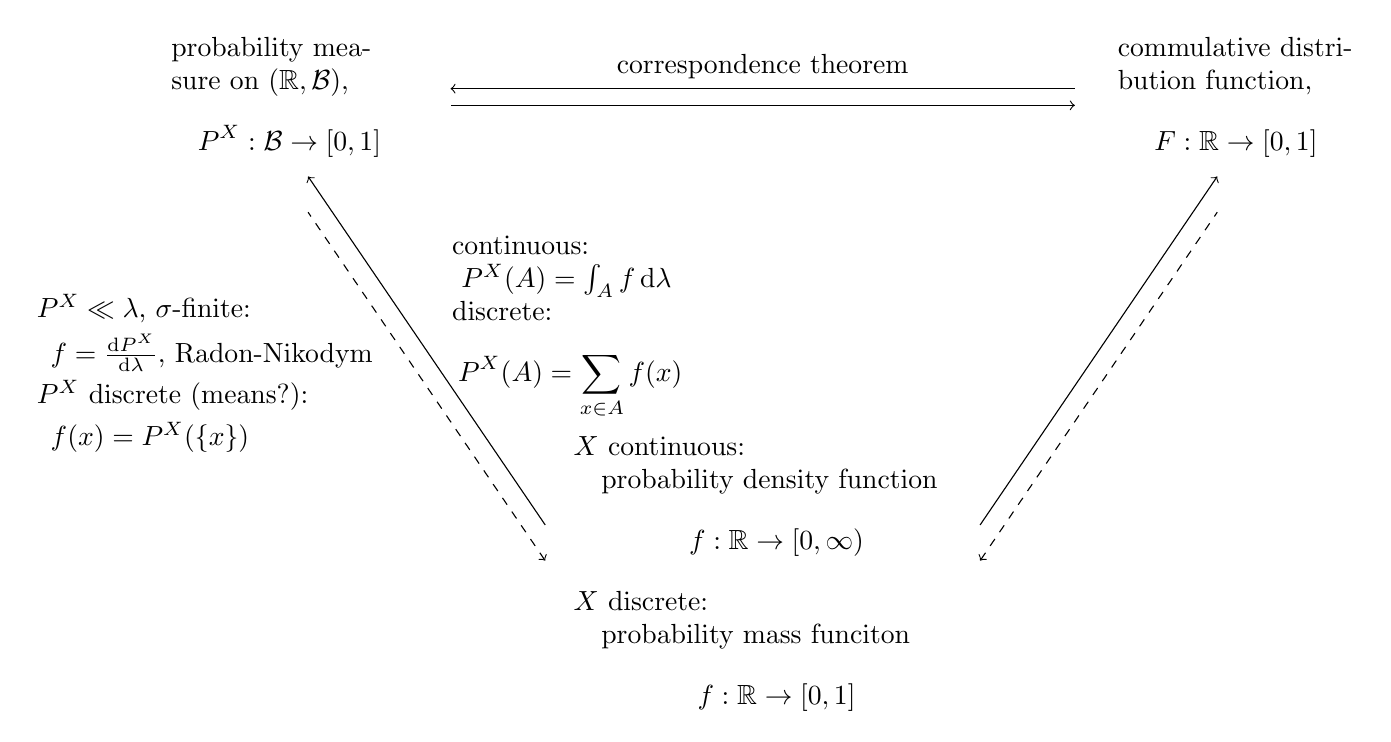
\begin{tikzpicture}[]
  \tikzstyle{equi} = [->,draw, shorten <=12pt, shorten >=12pt];
  
  \node (C) [text width=4.8cm, node distance = 6.5cm] {$X$ continuous: \\ \begin{addmargin}[1em]{0em} probability density function \[f: \mathbb{R} \to [0, \infty)\] \end{addmargin} $X$ discrete: \\ \begin{addmargin}[1em]{0em} probability mass funciton\[f:\mathbb{R} \to [0,1]\]\end{addmargin}};
  \node (A) [above right of=C, text width=3cm, node distance = 8.5cm] {commulative distribution function, \[F: \mathbb{R} \to [0,1]\]};
  \node (B) [above left of=C, text width=3cm, node distance = 8.5cm] {probability measure on $(\mathbb{R}, \mathcal{B})$, \[P^X: \mathcal{B} \to [0,1]\]};
  
  \tikzstyle{every path}=[equi]
  
  \draw[transform canvas={yshift=0.7ex},->] (A) -- node[anchor=west,above]{correspondence theorem} (B);  			
  \draw[transform canvas={yshift=-0.7ex},<-] (A) --  (B);
  \draw[transform canvas={yshift=1.5ex},<-] (B.270) -- node[right, text width=3cm, ,xshift=+0.2cm,yshift=0.3cm]{continuous:\\ $\, \, P^X(A) = \int_A f \,\mathrm{d}\lambda$\\discrete:\[P^X(A) = \sum_{x \in A} f(x)\]} (C.180);  			
  \draw[transform canvas={yshift=-1.5ex},<-, dashed]  (C.180) -- node[below, text width=4.5cm, ,xshift=-2.7cm,yshift=1.3cm]{$P^X \ll \lambda$, $\sigma$-finite:\\ \smallskip $\,\,\,f=\frac{\mathrm{d}P^X}{\mathrm{d}\lambda}$, Radon-Nikodym\\ \smallskip $P^X$ discrete (means?):\\ \smallskip $\,\,\,f(x) = P^X(\{x\})$}  (B.270);
  \draw[transform canvas={yshift=1.5ex},<-] (A.270) --  node[above]{} (C.0);  			
  \draw[transform canvas={yshift=-1.5ex},<-, dashed] (C.0) --  (A.270);

  
\end{tikzpicture}
  

\end{document}